\documentclass[11pt,a4paper]{jsarticle}

\usepackage{amsmath,amssymb}
\usepackage{bm}
\usepackage{graphicx}
\usepackage{ascmac}
\usepackage{subfigure}
\newlength{\subfigwidth}
\newlength{\subfigcolsep}

\graphicspath{{./img/}}

\title{TPC-H performance measure}
\author{Keisuke Suzuki}

\begin{document}
\maketitle
\section{実験環境}
\begin{itemize}
 \item CPU : Xeon X7560 @ 2.27GHz x4
 \item Memory : 64GB
 \item DBMS : PostgreSQL 9.2
 \item RAID0 : iodrive x8 (chunk size = 64KB)
 \item 各テーブルのprimary key上にB-tree indexを構築
 \item Scale Factor = 100
 \item shared buffer = 8GB
 \item 各クエリの実行時の状況をiostatとmpstatで1秒おきに監視
\end{itemize}

\clearpage
\section{Query 1 by index scan on l\_shipdate}
look-aheadを切った状態でのIO性能が乱れていたので、その原因を探る。

\subsection{random read microbenchmark}
測定時の条件
\begin{itemize}
 \item look-ahead (read-ahead): 0
 \item iosize: 8KB
 \item raw device access
\end{itemize}

\subsubsection{With O\_DIRECT flag}
まずOSのバッファリングなどを切った状態でのアクセス時の性能を示す。
\begin{figure}[thbp]
 \setlength{\subfigwidth}{.5\linewidth}
 \addtolength{\subfigwidth}{-.5\subfigcolsep}
 \begin{minipage}[b]{\subfigwidth}
  \subfigure[IOPS]{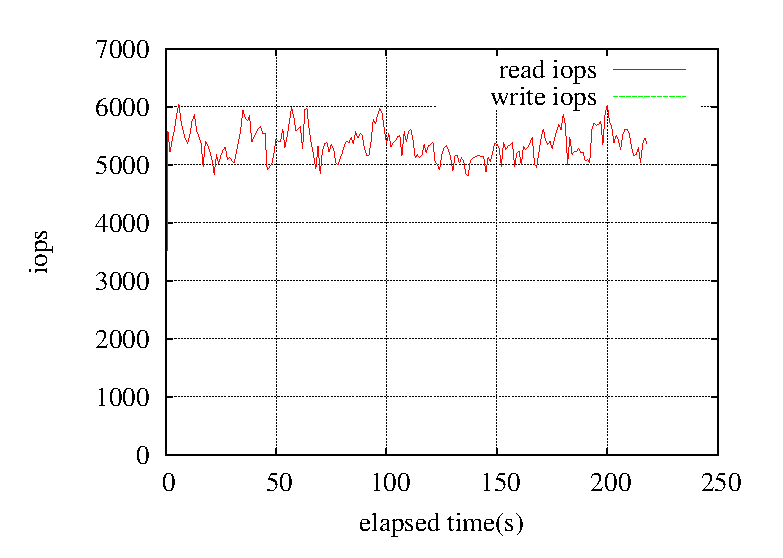
\includegraphics[width=75mm]{randomread_md0_8192_wodirectiops.eps}
  \label{fig:rand8192wodiops}}
 \end{minipage}
  \begin{minipage}[b]{\subfigwidth}
    \subfigure[iosize]{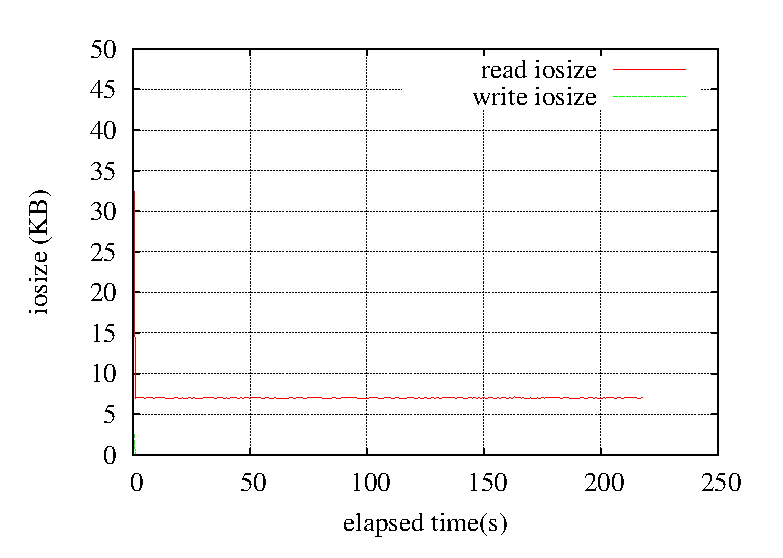
\includegraphics[width=75mm]{randomread_md0_8192_wodirectiosize.eps}
   \label{fig:rand8192wodiosize}}
  \end{minipage}
  \caption{IO spec (iosize = 8KB)}
  \label{fig:rand8192wod}
\end{figure}

\begin{table}[htbp]
 \begin{center}
  \caption{IO spec average (iosize = 8KB) \newline
  (IOPS = (io issued by benchmark / elapsed time))}
  \label{tbl:rand8192wod}
 \begin{tabular}{cc} \hline
  IOPS & MBPS \\ \hline
  4578 & 37.5 \\ \hline
 \end{tabular}
 \end{center}
\end{table}

\clearpage
benchmark実行時のIOの発行状況をblktraceで監視すると以下の通りであった。
\begin{verbatim}
  9,0    1        1     0.000000000 38969  Q   R 1894937090 + 16 [randomread]
  9,0    1        2     0.000011450 38969  U   N [randomread] 0
  9,0    1        3     0.000331059 38969  Q   R 1645272306 + 13 [randomread]
  9,0    1        4     0.000338372 38969  Q   R 1645272319 + 3 [randomread]
  9,0    1        5     0.000339942 38969  X   R 1645272319 / 1645272320 [randomread]
  9,0    1        6     0.000347454 38969  U   N [randomread] 0
  9,0    1        7     0.000611996 38969  Q   R 2143216519 + 16 [randomread]
  9,0    1        8     0.000615720 38969  U   N [randomread] 0
  ...
 CPU1 (md0):
 Reads Queued:       1,172K,    7,882MiB Writes Queued:           0,        0KiB
 Read Dispatches:        0,        0KiB  Write Dispatches:        0,        0KiB
 Reads Requeued:         0               Writes Requeued:         0
 Reads Completed:        0,        0KiB  Writes Completed:        0,        0KiB
 Read Merges:            0,        0KiB  Write Merges:            0,        0KiB
 Read depth:             0               Write depth:             0
 IO unplugs:      1,000,000              Timer unplugs:           0

Throughput (R/W): 0KiB/s / 0KiB/s
Events (md0): 2,273,525 entries
\end{verbatim}

\clearpage
\subsubsection{Without O\_DIRECT flag}
O\_DIRECT flagを使用しない状態でのアクセス時の性能を示す。
\begin{figure}[thbp]
 \setlength{\subfigwidth}{.5\linewidth}
 \addtolength{\subfigwidth}{-.5\subfigcolsep}
 \begin{minipage}[b]{\subfigwidth}
  \subfigure[IOPS]{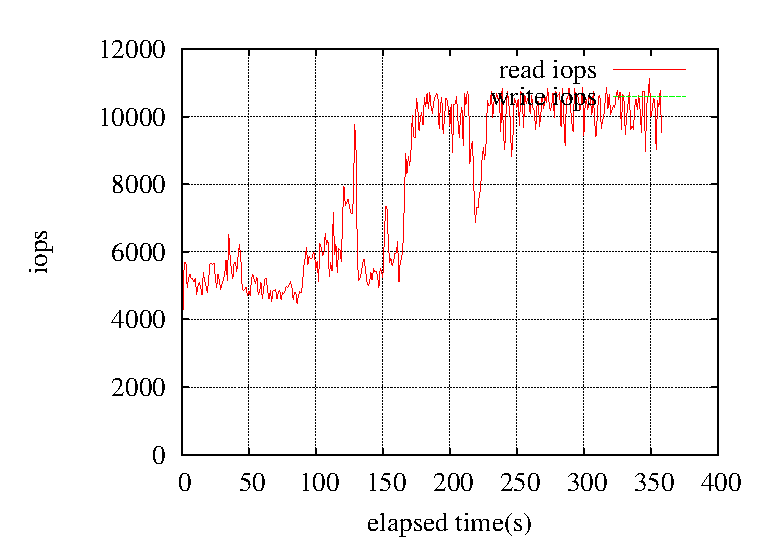
\includegraphics[width=75mm]{randomread_md0_8192iops.eps}
  \label{fig:rand8192iops}}
 \end{minipage}
  \begin{minipage}[b]{\subfigwidth}
    \subfigure[iosize]{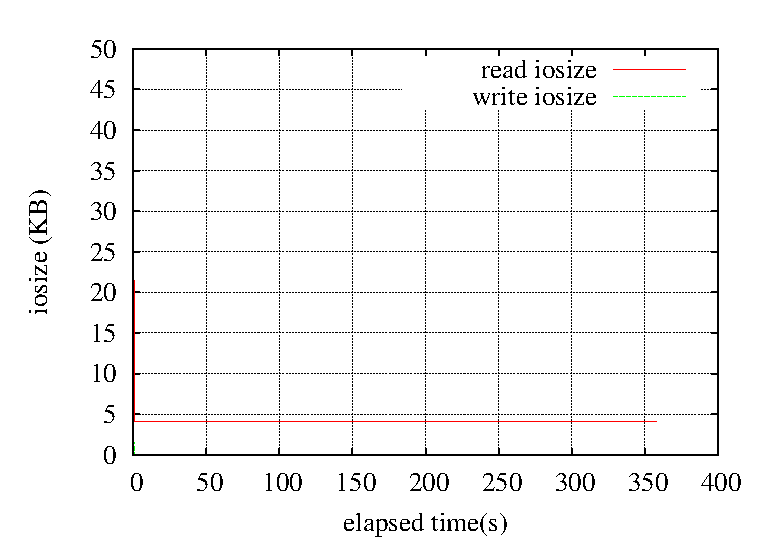
\includegraphics[width=75mm]{randomread_md0_8192iosize.eps}
   \label{fig:rand8192iosize}}
  \end{minipage}
  \caption{IO spec (iosize = 8KB)}
  \label{fig:rand8192}
\end{figure}

\begin{table}[htbp]
 \begin{center}
  \caption{IO spec average (iosize = 8KB) \newline
  (IOPS = (io issued by benchmark / elapsed time))}
  \label{tbl:rand8192}
 \begin{tabular}{cc} \hline
  IOPS & MBPS \\ \hline
  2787 & 22.8 \\ \hline
 \end{tabular}
 \end{center}
\end{table}

図\ref{fig:rand8192iosize}を見ると、クエリ実行時と同様の性能の乱れが見ら
れる。
この乱れは、iodriveをOSのbufferingを有効にして使用したときに生じる、デバ
イスの特性に由来するものではないかと考えられる。

また、iosizeに着目すると、本来8KBでIOを発行しているはずであるが、
実際のIOは半分の4KBで出ている。
iostatで計測したIOPSと、benchmarkで計算したIOPSも数値としてはあっていな
い。

そこでblktraceでbenchmark実行時のIOの発行状況を監視すると以下の通りであっ
た。

\clearpage
\begin{verbatim}
  9,0    1        1     0.000000000 39618  Q   R 1894937088 + 8 [randomread]
  9,0    1        2     0.000009686 39618  U   N [randomread] 0
  9,0    1        3     0.000274736 39618  Q   R 1894937096 + 8 [randomread]
  9,0    1        4     0.000278264 39618  U   N [randomread] 0
  9,0    1        5     0.000503299 39618  Q   R 1894937104 + 8 [randomread]
  9,0    1        6     0.000509047 39618  U   N [randomread] 0
  9,0    1        7     0.000794094 39618  Q   R 1645272304 + 8 [randomread]
  9,0    1        8     0.000800924 39618  U   N [randomread] 0
  9,0    1        9     0.001145873 39618  Q   R 1645272312 + 8 [randomread]
  9,0    1       10     0.001152079 39618  U   N [randomread] 0
  ...
CPU1 (md0):
 Reads Queued:       2,860K,   11,442MiB Writes Queued:           0,        0KiB
 Read Dispatches:        0,        0KiB  Write Dispatches:        0,        0KiB
 Reads Requeued:         0               Writes Requeued:         0
 Reads Completed:        0,        0KiB  Writes Completed:        0,        0KiB
 Read Merges:            0,        0KiB  Write Merges:            0,        0KiB
 Read depth:             0               Write depth:             0
 IO unplugs:      2,860,599              Timer unplugs:           0

Throughput (R/W): 0KiB/s / 0KiB/s
Events (md0): 5,721,230 entries
\end{verbatim}

この結果をみると、OSから発行されるIOは4KBのサイズになっている。
これはOSがページサイズ単位(4KB)にIOを分割して発行しているのではないかと
考えられる。
実際、他のサイズでIOを発行した場合も、OSからは4KBのIOとして発行されてい
ることが確認できた。
以下は、16KBのサイズでアクセスした場合の結果である。
\begin{verbatim}
  9,0    1        1     0.000000000 39810  Q   R 1894937088 + 8 [randomread]
  9,0    1        2     0.000008815 39810  U   N [randomread] 0
  9,0    1        3     0.000352988 39810  Q   R 1894937096 + 8 [randomread]
  9,0    1        4     0.000359066 39810  U   N [randomread] 0
  9,0    1        5     0.000656633 39810  Q   R 1894937104 + 8 [randomread]
  9,0    1        6     0.000662659 39810  U   N [randomread] 0
  ...
CPU1 (md0):
 Reads Queued:       4,831K,   19,327MiB Writes Queued:           0,        0KiB
 Read Dispatches:        0,        0KiB  Write Dispatches:        0,        0KiB
 Reads Requeued:         0               Writes Requeued:         0
 Reads Completed:        0,        0KiB  Writes Completed:        0,        0KiB
 Read Merges:            0,        0KiB  Write Merges:            0,        0KiB
 Read depth:             0               Write depth:             0
 IO unplugs:      4,831,926              Timer unplugs:           0

Throughput (R/W): 0KiB/s / 0KiB/s
Events (md0): 9,663,852 entries
\end{verbatim}
\end{document}
